\documentclass[10pt,a4paper]{book}

\title{机械原理(Mechanisms and Machine Theory)}
\author{魏舟}
\date{\today}

% ========== 基础宏包 ==========
\usepackage[table]{xcolor}
\usepackage{ctex}
\usepackage{geometry,graphicx,xcolor,color}
\usepackage{amssymb,amsmath,amsthm}
\usepackage{siunitx}
\usepackage{yhmath}
\usepackage{newpxtext,mathpazo}
\usepackage{newclude,ulem}
\usepackage{subcaption}
\usepackage{float}
\usepackage{tikz}
\usetikzlibrary{angles, quotes, arrows.meta}
\usepackage{enumerate}
\usepackage{enumitem}
\usepackage{wallpaper}
\usepackage{titlesec, titletoc}
\usepackage{fancyhdr}
\usepackage[colorlinks,linkcolor=winered]{hyperref}
\usepackage{xparse}

% ========== 颜色定义 ==========
\definecolor{winered}{rgb}{0.5,0,0}
\definecolor{structurecolor}{RGB}{122,122,142}
\definecolor{main}{rgb}{0.5,0,0}
\definecolor{second}{RGB}{115,45,2}
\definecolor{third}{RGB}{0,80,80}

% ========== tcolorbox 设置 ==========
\usepackage[skins, breakable, theorems, most]{tcolorbox}
\tcbuselibrary{theorems, breakable, skins, most}

\tcbset{
  mybox/.style = {
    enhanced, breakable,
    colback = white,
    colframe = #1!50!black,
    coltitle = white,
    fonttitle = \bfseries\kaishu,
    attach boxed title to top left = {yshift = -2mm, xshift = 3mm},
    boxed title style = {
      empty,
      boxrule = 0pt,
      colback = #1,
      rounded corners = north,
    },
    left = 3mm, right = 3mm, top = 3mm, bottom = 3mm,
    before skip = 12pt, after skip = 12pt,
    drop shadow,
    sharp corners,
  }
}

% ========== 重新定义 definition 环境（仿照手动示例） ==========
% 不带编号，标题为“定义：xxx”，蓝色直角盒子，浅蓝背景，支持跨页
\NewDocumentEnvironment{definition}{o}
  {%
    \IfNoValueTF{#1}
      {\begin{tcolorbox}[
          title=定义,
          colframe=blue!50!black,
          colback=blue!5!white,
          sharp corners,
          breakable,
          fonttitle=\bfseries\kaishu,
          before skip=12pt,
          after skip=12pt
        ]}
      {\begin{tcolorbox}[
          title=定义：#1,
          colframe=blue!50!black,
          colback=blue!5!white,
          sharp corners,
          breakable,
          fonttitle=\bfseries\kaishu,
          before skip=12pt,
          after skip=12pt
        ]}
  }
  {%
    \end{tcolorbox}
  }

% ========== 其他定理环境（使用 amsthm + tcolorboxenvironment） ==========
\newtheoremstyle{thmstyle}{3pt}{3pt}{\kaishu}{-3pt}{
  \bfseries\color{second}}{}{0.5em}{\indent【\thmname{#1} \thmnumber{#2}】 \thmnote{(#3)}}
\newtheoremstyle{prostyle}{3pt}{3pt}{\kaishu}{-3pt}{
  \bfseries\color{third}}{}{0.5em}{\indent【\thmname{#1} \thmnumber{#2}】 \thmnote{(#3)}}

\theoremstyle{thmstyle}
\newtheorem{theorem}{定理}[chapter]
\newtheorem{lemma}[theorem]{引理}
\newtheorem{corollary}[theorem]{推论}
\theoremstyle{prostyle}
\newtheorem{proposition}[theorem]{命题}
\newtheorem{example}[theorem]{例题}

% 为这些环境添加普通盒子（标题在内容区）
\tcolorboxenvironment{theorem}{mybox={second}}
\tcolorboxenvironment{lemma}{mybox={second}}
\tcolorboxenvironment{corollary}{mybox={second}}
\tcolorboxenvironment{proposition}{mybox={third}}
\tcolorboxenvironment{example}{mybox={structurecolor}}

% ========== 证明、解、注环境 ==========
\renewenvironment{proof}[1][证明]{\par{\kaishu \uline{\textbf{#1.}}} \;\fangsong}{\qed\par}
\newenvironment{solution}{\par\underline{\textbf{解.}} \;\kaishu}{\par}
\newenvironment{remark}{\par\underline{\textbf{注.}} \;\fangsong}{\par}
\newcommand{\intro}[1]{\rightline{\parbox[t]{5cm}{\footnotesize \fangsong\quad\quad #1 }}}

% ========== 其他样式 ==========
\setlist[enumerate,1]{label=\color{structurecolor}\arabic*.}
\setlist[enumerate,2]{label=\color{structurecolor}(\arabic*).}
\setlist[enumerate,3]{label=\color{structurecolor}\Roman*.}
\setlist[enumerate,4]{label=\color{structurecolor}\Alph*.}

\linespread{1.2}
\fancypagestyle{plain}{%
  \fancyhf{}
  \renewcommand{\headrulewidth}{0pt}
  \renewcommand{\footrulewidth}{0pt}
}

\titlecontents{chapter}[0em]{}{\large \fangsong{第 \thecontentslabel 章\quad}}{}{\hfill\contentspage}
\titlecontents{section}[2em]{}{\thecontentslabel\quad\textcolor{blue}}{}{\titlerule*{ .} \contentspage}

\titleformat{\chapter}[display]{\Large}
{\color{structurecolor}\centering\small \color{structurecolor}第 \zhnumber{\arabic{chapter}} \ 章 }{0.5ex}
{\color{structurecolor}{\titlerule[1pt]}\Large \kaishu \centering \bfseries}

\titleformat{\section}[frame]
{\normalfont\color{structurecolor}}
{\footnotesize \enspace \large \textcolor{structurecolor}{\S \,\thesection}\enspace}{6pt}
{\Large\filcenter \bf \kaishu }
\titlespacing*{\section}{1pc}{*7}{*2.3}[1pc]

\titleformat{\subsection}[hang]{\bfseries}{
  \large\bfseries\color{structurecolor}\thesubsection\enspace}{1pt}{%
  \color{structurecolor}\large\bfseries\filright}
\titleformat{\subsubsection}[hang]{\bfseries}{
  \large\bfseries\color{structurecolor}\thesubsubsection\enspace}{1pt}{%
  \color{structurecolor}\large\bfseries\filright}

\tikzset{
  joint/.style={circle, fill=black, minimum size=4pt, inner sep=0pt},
  link/.style={thick},
  fixed/.style={thick, double},
  arrow/.style={-{Stealth[scale=0.8]}}
}

% 可选：解决中文字体粗体缺失警告（使用 XeLaTeX）
% \setCJKmainfont{KaiTi}[AutoFakeBold=3]

\begin{document}
	
	\maketitle
	刚上大学，我的专业是机械工程学院的兵器类。在机械工程学院的一个月，我认识了很多很好的朋友。
	
	所以，我整理了一下机械原理课上的笔记，分享给我的同学，分享给我的热爱。
	\newpage
	
	\tableofcontents
	
	\setcounter{page}{0}
	\thispagestyle{empty}
	\newpage
	\chapter{导论(Introduction)}
\intro{凡筒井皆用机械，利之所在，人无不知。
}\rightline{——苏轼}

\section{研究对象}
{\Huge{Machinary(机械)}}————Machine(机器) and Mechanism(机构)

\subsection{机器的三个特征}
\begin{enumerate}
    \item 人为实物的组合
    \item 各组成部分间有确定的相互运动
    \item 能做有用功，完成信息的传递和能量的转换
\end{enumerate}

如果只满足前两个特征，就是机构，如果满足三个特征，就是机器。

\subsection{现代机械的组成}
\begin{enumerate}
    \item 原动机（Prime mover）
    \item 执行机构(Working system)
    \item 传动机构(Transmission system)
    \item 控制机构(Control system)
\end{enumerate}

\section{相关概念}
\subsection{构件}
\begin{definition}
    构件是一个机器的运动单元体，具有确定的运动。
\end{definition}
\subsubsection{构件的分类}
\begin{enumerate}
    \item 机架：固定不动的构件
    \item 原动件：驱动力（矩）作用的构件
    \item 从动件：随原动件运动而运动的构件
\end{enumerate}

\subsection{零件}
\begin{definition}
    零件是一个机器的制造单元体，不可拆分。
\end{definition}

\subsection{部件}
\begin{definition}
    为完成特定的功能在结构上组合在一起并协同工作的零件组合。
\end{definition}

	\chapter{平面机构的结构分析(Structure Analysis of Planar Mechanisms)}
\intro{有机械者必有机事，有机事者必有机心。}
\rightline{————《庄子》}


\section{机构结构分析的目的和内容}
\textbf{目的}：研究机构组成的共同规律，建立一般分析方法。

\section{机构的组成}
\subsection{平面机构和空间机构}
\begin{itemize}
    \item \textbf{空间机构}：至少有两个构件在三维空间作相对运动的机构。
    \item \textbf{平面机构}：组成机构的各构件均在同一平面内或相互平行的平面内运动。
\end{itemize}

\subsection{运动副 (Kinematic Pair)}
两构件直接接触，又能容许一定的相对运动的连接。

\begin{itemize}
    \item \textbf{低副 (Low Pair)}：面接触,提供两个约束
    \begin{enumerate}
        \item 转动副 (revolute pair)：1 DOF
        \begin{figure}[htbp]
            \centering
            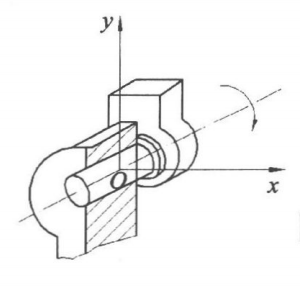
\includegraphics[width=0.2\textwidth]{figure/revolute_pair.png}
            \caption{转动副 (revolute pair)}
            \label{fig:revolute_pair}
        \end{figure}
        \item 移动副 (sliding pair)：1 DOF
        \begin{figure}[htbp]
            \centering
            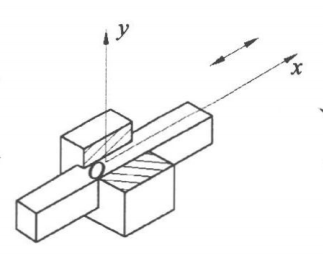
\includegraphics[width=0.2\textwidth]{figure/sliding_pair.png}
            \caption{移动副 (sliding pair)}
            \label{fig:sliding_pair}
        \end{figure}
    \end{enumerate}
    \item \textbf{高副 (High Pair)}：点/线接触,提供一个约束
    \begin{enumerate}
        \item 齿轮副 (gear pair)：2 DOF
        \begin{figure}[htbp]
            \centering
            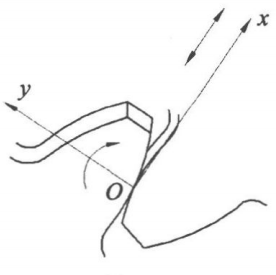
\includegraphics[width=0.2\textwidth]{figure/gear_pair.png}
            \caption{齿轮副 (gear pair)}
            \label{fig:gear_pair}
        \end{figure}
        \item 凸轮副 (cam pair)：2 DOF
        \begin{figure}[htbp]
            \centering
            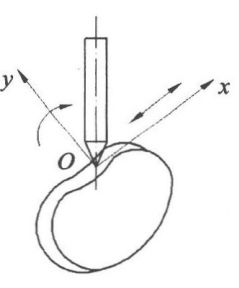
\includegraphics[width=0.2\textwidth]{figure/cam_pair.png}
            \caption{凸轮副 (cam pair)}
            \label{fig:cam_pair}
        \end{figure}
    \end{enumerate}
\end{itemize}

\subsubsection{自由度 (DOF)}
\begin{definition}
    构件含有独立运动的数目。
\end{definition}
\subsubsection{约束 (constraint)}
\begin{definition}
    对独立运动的限制。
\end{definition}

\subsection{运动链}
\begin{definition}
    两个以上的构件由运动副连接而成的系统。
\end{definition}

\begin{itemize}
    \item \textbf{闭链 (Closed chain)}
    \begin{definition}
        形成封闭回路的运动链。
\end{definition}
    \item \textbf{开链 (Open chain)}
    \begin{definition}
        未形成封闭回路的运动链。
\end{definition}
\end{itemize}
\[
\text{构件} + \text{运动副} = \text{运动链}
\]
\begin{remark}
    一个机构只有一个机架！
\end{remark}

\section{机构的运动简图 (Kinematic Diagram of Mechanism)}
\begin{remark}
    机构示意图和机构运动简图的区别：
    机构示意图只代表构件和运动副，不考虑运动副的相对位置。
    机构运动简图则考虑运动副的相对位置，更详细地表示机构的运动规律。
\end{remark}
\subsection{运动副表示方法}
\begin{enumerate}
    \item \textbf{转动副}  \textbf{轴线正确位置}：用圆圈表示转动中心，绘制两构件的相对位置。
    \begin{figure}[htbp]
        \centering
        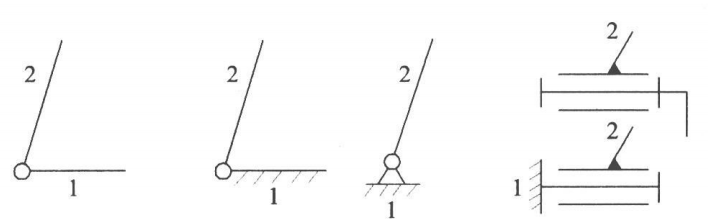
\includegraphics[width=0.5\textwidth]{figure/revolute_pair_draw.png}
        \caption{转动副运动简图}
    \end{figure}
    \item \textbf{移动副}  \textbf{相对移动方向}：用导路和滑块表示，突出移动方向。
    \begin{figure}[htbp]
        \centering
        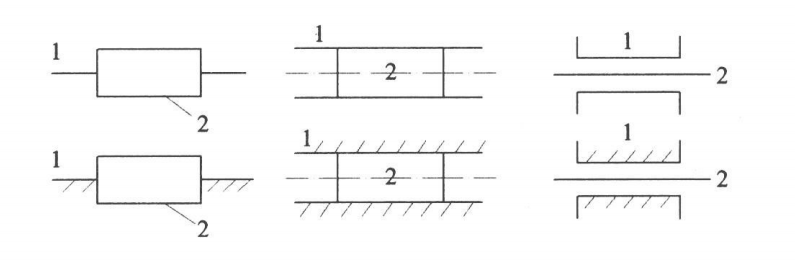
\includegraphics[width=0.5\textwidth]{figure/sliding_pair_draw.png}
        \caption{移动副运动简图}
    \end{figure}
    \item \textbf{齿轮副}  \textbf{相互接触部分}：用节圆或啮合线表示齿轮的啮合关系。
    \begin{figure}[htbp]
        \centering
        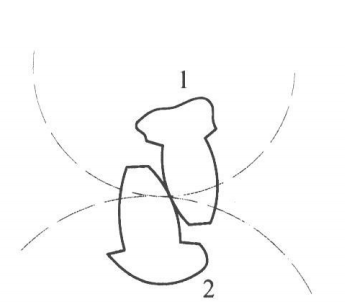
\includegraphics[width=0.5\textwidth]{figure/gear_pair_draw.png}
        \caption{齿轮副运动简图}
    \end{figure}
    \item \textbf{凸轮副}  \textbf{相互接触的曲线轮廓}：绘制凸轮轮廓与从动件的接触形态。
    \begin{figure}[htbp]
        \centering
        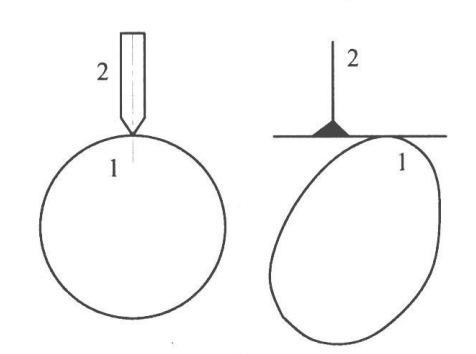
\includegraphics[width=0.5\textwidth]{figure/cam_pair_draw.png}
        \caption{凸轮副运动简图}
    \end{figure}
\end{enumerate}

\subsection{构件的表示方式}
不考虑与运动无关的因素（如无关外形等），核心是表达构件间的连接关系。
原则：会画就会看，会看就会画。

\subsection{画机构运动简图的一般步骤}
\begin{figure}[htbp]
    \centering
    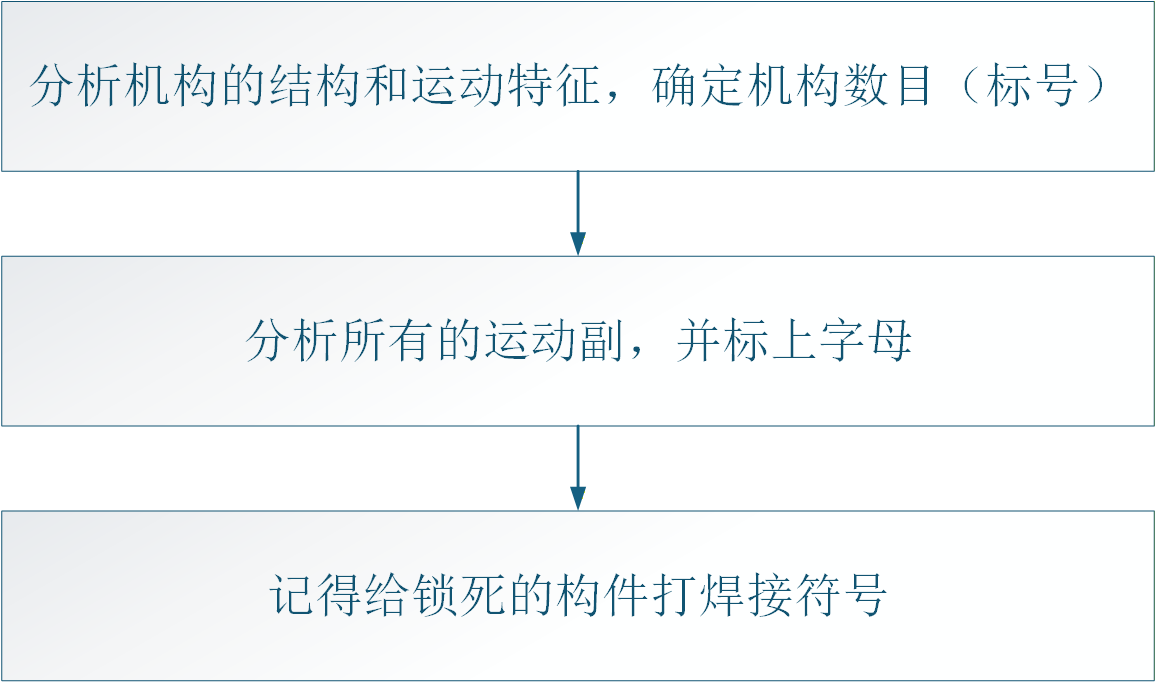
\includegraphics[width=0.5\textwidth]{figure/机构简图绘制流程.png}
    \caption{机构运动简图的一般步骤}
\end{figure}
\section{机构的自由度}
平面机构自由度计算公式：
\[
DOF = 3n - 2P_L - P_H
\]
其中：
\begin{itemize}
    \item \(n\)：活动构件个数
    \item \(P_L\)：低副个数
    \item \(P_H\)：高副个数
\end{itemize}

\subsubsection{机构具有确定运动的条件}：
\[
\begin{cases}
DOF > 0 \\
\text{原动件数} = \text{机构的自由度}
\end{cases}
\]

\subsection{复合铰链(Compound Hinge)}
\(k\) 个构件组成的复合铰链，应将 \(k-1\) 个转动副计入计算。

\subsection{局部自由度(Passive DOF)}
存在与否不影响整个机构的运动规律，计算自由度之前先去除局部自由度（常为滚轮结构）。处理方法：焊死即可。

\subsection{虚约束 (Redundant Constraints)}
某些约束对机构的限制作用或自由度的影响是重复的，即不起独立限制作用的约束。计算时需摘掉构件和约束（有限定几何条件，一般情况）。

\subsection{常见情况}
\begin{enumerate}
    \item 不同构件上两点间距、距离保持恒定。
    \item 两构件构成多个移动副且导路互相平行。
    \item 两构件构成多个转动副且轴线相互重合。
    \item 在输入件与输出件之间用多组完全相同的运动链来传递运动，只有一组起独立传递运动的作用，其余引入虚约束。
\end{enumerate}

\section{自由度计算的步骤}
\begin{figure}[htbp]
    \centering
    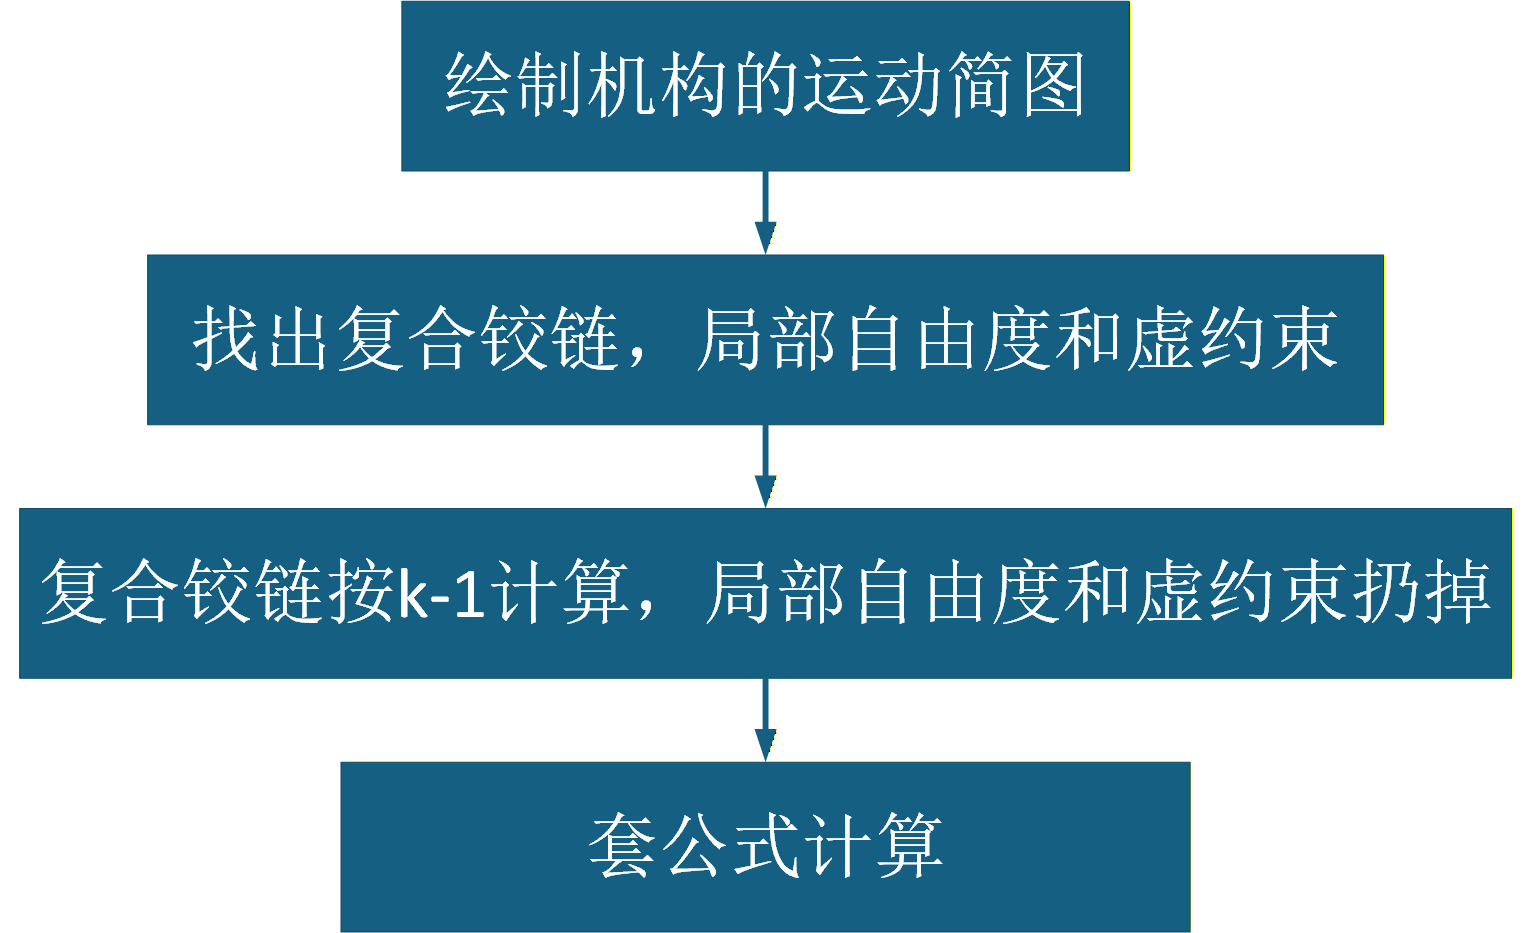
\includegraphics[width=0.8\textwidth]{figure/自由度计算步骤.png}
    \caption{自由度计算的步骤}
\end{figure}

	\chapter{机构运动分析}
	
	在机构运动分析中，速度分析是核心任务之一。瞬心法（Instant Center Method）是一种基于几何运动学的解析与作图相结合的方法，特别适用于简单平面机构的速度分析。
	
	\section{瞬心法}
	
	\subsection{瞬心的定义}
	**速度瞬心**（简称瞬心）是指两个处于相对运动中的构件，在任一瞬时其相对速度为零的重合点。
	\begin{itemize}
		\item \textbf{绝对瞬心}：若其中一个构件为机架（静止不动），则该点在该瞬时的绝对速度为零。
		\item \textbf{相对瞬心}：若两个构件都在运动，则该点在该瞬时具有相同的绝对速度（即相对速度为零）。
	\end{itemize}
	
	\subsection{瞬心的数量}
	对于一个由 $n$ 个构件（包含机架）组成的机构，由于任意两个构件之间都存在一个瞬心，其瞬心总数 $K$ 可以通过组合公式计算：
	\begin{equation}
		K = \binom{n}{2} = \frac{n(n-1)}{2}
	\end{equation}
	例如：对于常见的四杆机构 ($n=4$)，瞬心总数为 $K = \frac{4 \times 3}{2} = 6$ 个。
	
	\subsection{运动副的瞬心}
	通过运动副直接相连的两个构件，其瞬心位置可以直接确定：
	\begin{enumerate}
		\item \textbf{转动副}：瞬心就在转动副的中心点。
		\item \textbf{移动副}：两构件的相对运动为直线移动，其瞬心位于垂直于移动方向的无穷远处 ($P \to \infty$)。
		\item \textbf{平面高副（纯滚动）}：两构件接触点即为瞬心。
		\item \textbf{平面高副（滚动兼滑动）}：瞬心位于接触点处的公法线上，具体位置需结合其他约束确定。
	\end{enumerate}
	
	\subsection{三心定理}
	对于不直接相连的构件，其瞬心位置通常利用三心定理来确定。
	
	\begin{theorem}[三心定理]
		三个彼此作平面运动的构件，其三个共有瞬心必定位于同一直线上。
	\end{theorem}
	
	\textbf{证明简述}：
	设三个构件分别为 1, 2, 3。瞬心 $P_{12}$ 和 $P_{13}$ 已知。假设瞬心 $P_{23}$ 是构件 2 和 3 的重合点。
	\begin{itemize}
		\item 作为构件 2 上的点，其速度 $v_{P23}$ 应垂直于连线 $P_{12}P_{23}$；
		\item 作为构件 3 上的点，其速度 $v_{P23}$ 应垂直于连线 $P_{13}P_{23}$。
	\end{itemize}
	若要使 $v_{P23}$ 为同一矢量（大小相等且方向相同），则 $P_{12}$、$P_{13}$ 和 $P_{23}$ 必须共线。
	
	\subsection{瞬心法的应用}
	利用瞬心法求机构的速度，通常遵循以下步骤：
	\begin{enumerate}
		\item 计算机构的瞬心总数 $K$。
		\item 标出所有通过运动副直接确定的“显见瞬心”。
		\item 利用三心定理，通过作图法（连线交点）找出待求的“隐藏瞬心”。
		\item 根据公式 $v = \omega \cdot r$ 进行速度换算。例如，已知构件 1 的角速度 $\omega_1$，求构件 3 的角速度 $\omega_3$：
		\begin{equation}
			v_{P13} = \omega_1 \cdot l_{P12P13} = \omega_3 \cdot l_{P32P13}
		\end{equation}
	\end{enumerate}


\section{相对运动图解法（矢量方程图解法）}

相对运动图解法是基于多刚体运动学中的速度和加速度合成定理，通过列出矢量方程并利用几何作图（速度图、加速度图）求解未知量的方法。

\subsection{基本原理}
设构件上点 $A$ 为已知运动点，点 $B$ 为待求点，则其运动关系为：
\begin{itemize}
	\item \textbf{速度矢量方程}：$\vec{v}_B = \vec{v}_A + \vec{v}_{BA}$
	\item \textbf{加速度矢量方程}：$\vec{a}_B = \vec{a}_A + \vec{a}_{BA}^n + \vec{a}_{BA}^t$
\end{itemize}
其中，$\vec{v}_{BA}$ 垂直于连线 $AB$，$\vec{a}_{BA}^n$（法向加速度）指向旋转中心，$\vec{a}_{BA}^t$（切向加速度）垂直于连线 $AB$。

\subsection{哥氏加速度 (Coriolis Acceleration)}
当动点在转动的导路（动坐标系）上移动时，必须考虑哥氏加速度：
\begin{equation}
	\vec{a}_k = 2\vec{\omega} \times \vec{v}_{rel}
\end{equation}
其大小为 $a_k = 2\omega v_{rel}$，方向判定遵循左手法则或将 $\vec{v}_{rel}$ 沿 $\vec{\omega}$ 方向旋转 $90^\circ$。

\subsection{速度图与加速度图的特性}
\begin{enumerate}
	\item \textbf{速度极点 $p$}：图中所有从极点出发的矢量代表绝对速度，连接两点间的矢量代表相对速度。
	\item \textbf{速度影像原理}：同一构件上各点在速度图（或加速度图）中所组成的图形，与原构件上各点组成的几何图形相似，且字母顺序一致，旋转方向一致。
\end{enumerate}

\section{解析法（矢量方程解析法）}

解析法通过建立坐标系，利用机构的封闭矢量环方程进行求导，从而获得运动参数的精确解析解，是计算机辅助机构设计（CAMS）的基础。

\subsection{复数矢量法}
将构件看作复平面上的矢量，构件长度为 $l_i$，与 $x$ 轴夹角为 $\phi_i$。对于一个四杆机构，其封闭矢量环方程为：
\begin{equation}
	l_1 e^{j\phi_1} + l_2 e^{j\phi_2} = l_3 e^{j\phi_3} + l_4 e^{j\phi_4}
\end{equation}

\subsection{方程求解步骤}
\begin{enumerate}
	\item \textbf{位姿分析}：利用欧拉公式 $e^{j\phi} = \cos\phi + j\sin\phi$ 将矢量方程展开为实部（$x$ 轴）和虚部（$y$ 轴）的两个代数方程，解出未知的角位置 $\phi$。
	\item \textbf{速度分析}：对位姿方程关于时间 $t$ 求一阶导数：
	\begin{equation}
		\sum_{i=1}^n j l_i \omega_i e^{j\phi_i} = 0
	\end{equation}
	\item \textbf{加速度分析}：对速度方程关于时间 $t$ 再求一次导数：
	\begin{equation}
		\sum_{i=1}^n (j l_i \alpha_i e^{j\phi_i} - l_i \omega_i^2 e^{j\phi_i}) = 0
	\end{equation}
\end{enumerate}

\subsection{解析法的优点}
相比图解法，解析法能够：
\begin{itemize}
	\item 提供极高的计算精度。
	\item 易于编写程序进行全行程的运动特性曲线绘制。
	\item 方便进行机构的优化设计。
\end{itemize}
	\chapter{连杆机构(Planar Linkage Mechanisms)}
平面连杆机构是由若干刚性构件通过低副（转动副、移动副）连接而成，在同一平面或相互平行平面内运动的机构，广泛应用于工程机械、机床、汽车等领域。

\section{四杆机构(Four-bar Linkages)}
四杆机构是平面连杆机构中最基本、应用最广泛的机构，由四个刚性构件通过低副连接组成。

\subsection{四杆机构的基本类型}
四杆机构的最基本类型就是\textbf{铰链四杆机构}（四个连接副均为转动副）。
根据连架杆能否做整周转动，铰链四杆机构分为以下三类：

\subsubsection{1. 曲柄摇杆机构 (Crank-rocker Mechanism)}
- 定义：两连架杆中，一个为曲柄（能做360°整周转动），一个为摇杆（仅做往复摆动）。


- 应用：雷达天线俯仰机构、缝纫机踏板机构。

\begin{figure}[H]
	\centering
	\begin{tikzpicture}[scale=1.5]
		% 四个节点：A(机架左), B(曲柄端), C(连杆), D(机架右)
		\coordinate (A) at (0,0);
		\coordinate (D) at (3,0);
		\coordinate (B) at (1,1.2);
		\coordinate (C) at (2.2,0.8);
		% 绘制构件
		\draw[fixed] (A) -- (D) node[midway, below] {机架($d$)};
		\draw[link, red] (A) -- (B) node[midway, left] {曲柄($a$)};
		\draw[link, blue] (B) -- (C) node[midway, above] {连杆($b$)};
		\draw[link, green] (C) -- (D) node[midway, right] {摇杆($c$)};
		% 绘制铰链
		\foreach \p in {A,B,C,D} \fill[black] (\p) circle (2pt);
		\node at (A)[below left] {$A$};
		\node at (B)[above left] {$B$};
		\node at (C)[above right] {$C$};
		\node at (D)[below right] {$D$};
	\end{tikzpicture}
	\caption{曲柄摇杆机构}
\end{figure}

\subsubsection{2. 双曲柄机构 (Double-crank Mechanism)}
- 定义：两连架杆\textbf{均为曲柄}，均可做360°整周转动。
- 特殊形式：**平行双曲柄机构**（对边构件长度相等，两曲柄转速相同）。
- 应用：机车车轮联动机构、摄影升降平台。

\begin{figure}[H]
	\centering
	\begin{tikzpicture}[scale=1.5]
		\coordinate (A) at (0,0);
		\coordinate (D) at (3,0);
		\coordinate (B) at (0,2);
		\coordinate (C) at (3,2);
		\draw[fixed] (A) -- (D) node[below] {机架($d$)};
		\draw[link, red] (A) -- (B) node[left] {主动曲柄($a$)};
		\draw[link] (B) -- (C) node[above] {连杆($b$)};
		\draw[link, red] (C) -- (D) node[right] {从动曲柄($c$)};
		\foreach \p in {A,B,C,D} \fill[black] (\p) circle (2pt);
	\end{tikzpicture}
	\caption{平行双曲柄机构}
\end{figure}

\subsubsection{3. 双摇杆机构 (Double-rocker Mechanism)}
- 定义：两连架杆\textbf{均为摇杆}，只能做往复摆动，无曲柄存在。
- 应用：起重机变幅机构、电风扇摇头机构。

\begin{figure}[H]
	\centering
	\begin{tikzpicture}[scale=1.5]
		\coordinate (A) at (0,0);
		\coordinate (D) at (3,0);
		\coordinate (B) at (0.8,1.5);
		\coordinate (C) at (2.2,1.5);
		\draw[fixed] (A) -- (D) node[below] {机架($d$)};
		\draw[link, green] (A) -- (B) node[left] {摇杆($a$)};
		\draw[link] (B) -- (C) node[above] {连杆($b$)};
		\draw[link, green] (C) -- (D) node[right] {摇杆($c$)};
		\foreach \p in {A,B,C,D} \fill[black] (\p) circle (2pt);
	\end{tikzpicture}
	\caption{双摇杆机构}
\end{figure}

\subsubsection{4. 含有移动副的四杆机构（衍生类型）}
在铰链四杆机构基础上，将转动副转化为移动副，得到：
\begin{enumerate}[itemsep=2pt]
	\item 曲柄滑块机构（内燃机、压缩机核心机构）
	\item 导杆机构
	\item 摇块机构
	\item 定块机构
\end{enumerate}

\section{平面连杆机构的运动特性}
\subsection{曲柄存在条件}
铰链四杆机构中，**连架杆成为曲柄的充要条件**：

\subsubsection{1. 杆长条件（格拉霍夫定理 Grashof's Law）}
设：
\begin{itemize}
	\item 最短杆长度：$a$
	\item 最长杆长度：$d$
	\item 其余两杆长度：$b、c$
\end{itemize}
满足：
\[
\boldsymbol{\text{最短杆长度 + 最长杆长度} \leq \text{其余两杆长度之和}}
\]
即：
\[
a + d \leq b + c
\]

\subsubsection{2. 机架条件}
\begin{enumerate}[itemsep=2pt]
	\item 最短杆为\textbf{连架杆} $\rightarrow$ 曲柄摇杆机构
	\item 最短杆为\textbf{机架} $\rightarrow$ 双曲柄机构
	\item 最短杆为\textbf{连杆} $\rightarrow$ 双摇杆机构
	\item 若不满足杆长条件 $\rightarrow$ 无论哪个杆为机架，均为双摇杆机构
\end{enumerate}

\subsection{压力角和传动角}
压力角与传动角是衡量机构**传力性能**的核心指标。

\subsubsection{1. 定义}
- **压力角$\boldsymbol{\alpha}$**：从动件上受力点的速度方向与受力方向之间的锐角。
- **传动角$\boldsymbol{\gamma}$**：压力角的余角，$\boldsymbol{\gamma = 90^\circ - \alpha}$。
- 关系：$\gamma$ 越大，$\alpha$ 越小，机构传力性能越好。

\begin{figure}[H]
	\centering
	\begin{tikzpicture}[scale=1.8]
		\coordinate (A) at (0,0);
		\coordinate (D) at (3,0);
		\coordinate (B) at (1,1);
		\coordinate (C) at (2.2,0.8);
		% 机构
		\draw[fixed] (A)--(D);
		\draw[link] (A)--(B) (B)--(C) (C)--(D);
		% 压力角/传动角标注
		\draw[arrow, red] (C) -- +(0.6,0) node[right] {速度方向};
		\draw[arrow, blue] (C) -- (B) node[midway, above] {受力方向};
		\pic[draw, "$\alpha$", angle radius=10pt] {angle=B--C--D};
		\pic[draw, "$\gamma$", angle radius=15pt] {angle=D--C--B};
		\foreach \p in {A,B,C,D} \fill (\p) circle (2pt);
	\end{tikzpicture}
	\caption{压力角$\alpha$与传动角$\gamma$}
\end{figure}

\subsubsection{2. 设计要求}
工程上通常要求：
\[
\gamma_{\text{min}} \geq 40^\circ \sim 50^\circ
\]

\subsection{行程变化系数（行程速比系数$K$）}
用于描述机构的**急回特性**（从动件回程速度大于工作行程速度）。

\subsubsection{1. 极位夹角$\boldsymbol{\theta}$}
曲柄摇杆机构中，摇杆处于**两个极限位置**时，曲柄对应的两位置之间的夹角$\theta$。

\subsubsection{2. 行程速比系数公式}
\[
\boldsymbol{K = \frac{180^\circ + \theta}{180^\circ - \theta}}
\]
- $K>1$：机构具有急回特性

- $K=1$：无急回特性

- $\theta$ 越大，$K$ 越大，急回特性越明显

\subsubsection{3. 极位夹角求解公式}
\[
\theta = \frac{K-1}{K+1} \times 180^\circ
\]

\begin{figure}[H]
	\centering
	\begin{tikzpicture}[scale=1.6]
		\coordinate (A) at (0,0);
		\coordinate (D) at (3,0);
		\coordinate (C1) at (1.5,1.8);
		\coordinate (C2) at (2.5,1.0);
		\coordinate (B1) at (0.6,0.8);
		\coordinate (B2) at (-0.5,0.3);
		% 极限位置
		\draw[fixed] (A)--(D);
		\draw[dashed, link] (A)--(B1) (B1)--(C1) (C1)--(D);
		\draw[dashed, link] (A)--(B2) (B2)--(C2) (C2)--(D);
		\draw[red, thick] (B2)--(A)--(B1);
		\pic[draw, "$\theta$", angle radius=20pt] {angle=B2--A--B1};
		\foreach \p in {A,D,C1,C2} \fill (\p) circle (2pt);
	\end{tikzpicture}
	\caption{极位夹角$\theta$}
\end{figure}

\subsection{死点}
\subsubsection{1. 定义}
在曲柄摇杆机构中，当**连杆与从动曲柄共线**时，机构的传动角$\gamma=0^\circ$，压力角$\alpha=90^\circ$，此时主动力无法推动机构运动，该位置称为**死点位置**。

\subsubsection{2. 死点位置特征}
- 传动角 $\boldsymbol{\gamma=0^\circ}$
- 机构传力力矩为0
- 机构可能出现运动不确定、卡死现象

\subsubsection{3. 死点位置的应用与克服}
\begin{enumerate}[itemsep=2pt]
	\item \textbf{利用死点}：夹具、飞机起落架（利用死点实现自锁，保持位置固定）
	\item \textbf{克服死点}：
	\begin{itemize}
		\item 加装飞轮（利用惯性通过死点，如蒸汽机、内燃机）
		\item 多组机构错位排列（如机车车轮）
	\end{itemize}
\end{enumerate}

\begin{figure}[H]
	\centering
	\begin{tikzpicture}[scale=1.5]
		\coordinate (A) at (0,0);
		\coordinate (D) at (3,0);
		\coordinate (B) at (1,0);
		\coordinate (C) at (2,0);
		% 死点：曲柄与连杆共线
		\draw[fixed] (A)--(D);
		\draw[link, red] (A)--(B);
		\draw[link, blue] (B)--(C);
		\draw[link, green] (C)--(D);
		\foreach \p in {A,B,C,D} \fill[black] (\p) circle (2pt);
		\node at (1.5, 0.3) {死点位置（共线）};
	\end{tikzpicture}
	\caption{四杆机构死点位置}
\end{figure}

\section{四杆机构的设计}
平面四杆机构设计，是根据给定运动规律、轨迹要求或极限位置，确定各构件杆长、铰链位置的综合过程。
常用设计方法分为：\textbf{图解法}、\textbf{解析法}。

\subsection{图解法}
图解法几何直观、作图简便，适合按给定连杆位置、摇杆摆角、急回系数等条件设计四杆机构，核心基础为\textbf{刚体倒置思想（反转法/机架变换法）}。

\subsubsection{刚体倒置思想（反转法原理）}
\label{sec:inversion}
刚体倒置基本思路：
给整个机构施加一个**公共反向角速度**，机构各构件间相对运动关系保持不变，仅改变机架，将「连架杆运动问题」转化为「连杆定点轨迹问题」。

核心要点：
\begin{enumerate}
	\item 平面机构相对运动与机架选取无关；
	\item 固定原主动件，把原机架视为运动构件，实现运动倒置；
	\item 利用倒置后铰链定点圆周轨迹，图解求得铰链中心位置。
\end{enumerate}

适用典型设计工况：
\begin{itemize}
	\item 按给定两连架杆对应转角设计四杆机构；
	\item 按给定连杆三个位置设计铰链四杆机构；
	\item 按行程速比系数 $K$ 设计曲柄摇杆机构。
\end{itemize}

\subsubsection{按急回系数 $K$ 图解设计曲柄摇杆机构}
设计步骤：
\begin{enumerate}
	\item 由已知 $K$ 计算极位夹角：
	\[
	\theta = 180^\circ \cdot \dfrac{K-1}{K+1}
	\]
	\item 选定摇杆长度 $l_{CD}$ 及摆角 $\psi$，作出摇杆两极限位置 $C_1D$、$C_2D$；
	\item 作 $C_1C_2$ 连线，作辅助圆使得圆周角为 $\theta$；
	\item 曲柄回转中心 $A$ 落在该圆周上，选定 $A$ 点；
	\item 由几何关系求曲柄长 $a$、连杆长 $b$：
	\[
	\begin{cases}
		l_{AC_1} = b - a\\
		l_{AC_2} = b + a
	\end{cases}
	\]
	联立解得：
	\[
	a = \dfrac{l_{AC_2}-l_{AC_1}}{2},\quad 
	b = \dfrac{l_{AC_2}+l_{AC_1}}{2}
	\]
\end{enumerate}

\begin{figure}[H]
	\centering
	\begin{tikzpicture}[scale=1.4,
		joint/.style={circle,fill=black,minimum size=3pt,inner sep=0pt},
		link/.style={thick},
		fixed/.style={thick,double}]
		% 机架D
		\coordinate (D) at (4,0);
		\coordinate (C1) at (1.5,1.8);
		\coordinate (C2) at (2.8,1.2);
		\coordinate (A) at (0,0);
		
		% 摇杆两极限位置
		\draw[link] (D) -- (C1) node[above] {$C_1$};
		\draw[link] (D) -- (C2) node[above] {$C_2$};
		\draw[fixed] (A) -- (D) node[midway,below] {机架};
		
		% 连线
		\draw[dashed] (C1) -- (C2);
		\draw[dashed,red] (A) -- (C1);
		\draw[dashed,red] (A) -- (C2);
		
		% 极位夹角
		\pic[draw,"$\theta$",angle radius=18pt,angle eccentricity=1.3] {angle=C1--A--C2};
		% 摆角
		\pic[draw,"$\psi$",angle radius=15pt] {angle=C2--D--C1};
		
		\foreach \p in {A,D,C1,C2} \node[joint] at (\p) {};
		\node[below left] at (A) {$A$};
		\node[below right] at (D) {$D$};
	\end{tikzpicture}
	\caption{按急回系数 $K$ 图解设计曲柄摇杆机构}
\end{figure}

\subsubsection{按给定连杆位置设计（刚体倒置应用）}
给定连杆 $BC$ 两个/三个位置，利用反转法：
把连杆视为固定机架，原机架 $AD$ 变为运动连杆，作铰链 $A$、$D$ 所在圆心，几何作图直接求得各杆长度。

\subsection{解析法}
图解法精度受作图误差限制，\textbf{解析法}通过建立闭环矢量方程、坐标几何关系，精确求解各构件杆长与铰链坐标，适合工程高精度设计与计算机编程求解。

\subsubsection{闭环矢量建模}
将铰链四杆机构视为封闭矢量多边形：
设四杆矢量依次为：机架 $\vec{l_4}$、曲柄 $\vec{l_1}$、连杆 $\vec{l_2}$、摇杆 $\vec{l_3}$，满足闭环条件：
\[
\vec{l_1} + \vec{l_2} = \vec{l_4} + \vec{l_3}
\]

建立直角坐标系，将矢量分解为 $x,y$ 分量：
\[
\begin{cases}
	l_1\cos\varphi_1 + l_2\cos\varphi_2 = l_4 + l_3\cos\varphi_3\\
	l_1\sin\varphi_1 + l_2\sin\varphi_2 = l_3\sin\varphi_3
\end{cases}
\]
$\varphi_1$ 为曲柄转角，$\varphi_2$ 连杆角，$\varphi_3$ 摇杆摆角。

\subsubsection{位移、角位移解析关系}
消去中间连杆角 $\varphi_2$，整理可得**曲柄—摇杆角位移关系式**：
\[
\cos\varphi_3 = P_1\cos\varphi_1 + P_2\cos(\varphi_1-\varphi_3) + P_3
\]
其中 $P_1,P_2,P_3$ 为仅与各杆杆长有关的结构参数。

给定多组曲柄、摇杆对应转角，代入方程可构造方程组，**求解四杆机构各杆相对长度**。

\subsubsection{解析法设计特点}
\begin{enumerate}
	\item 计算精度高，无作图误差；
	\item 适合多位置精确逼近、优化设计；
	\item 便于编程实现、参数化建模与CAD二次开发；
	\item 可结合最小传动角、空间约束进行优化设计。
\end{enumerate}

\subsubsection{常用设计工况解析求解}
\begin{itemize}
	\item 给定两连架杆三组对应转角，精确求解杆长比例；
	\item 给定摇杆摆角、极位夹角，解析求曲柄、连杆、机架长度；
	\item 约束最小传动角，进行四杆机构优化设计。
\end{itemize}
	\chapter{凸轮机构 (Cam Mechanisms)}

\intro{凸轮机构是由凸轮、从动件和机架三个基本构件组成的高副机构。它能将凸轮的连续转动转化为从动件预期的往复移动或摆动。}

\section{凸轮机构的应用和分类}

\subsection{凸轮机构的应用}
凸轮机构的主要优点是只需设计适当的凸轮轮廓曲线，就可以使从动件实现任意给定的运动规律，且结构紧凑、易于设计。常见于：
\begin{itemize}
	\item 内燃机配气机构
	\item 自动机床的进给机构
	\item 工业机器人的控制机构
\end{itemize}

\subsection{凸轮机构的分类}

\begin{enumerate}
	\item \textbf{按凸轮形状分类}：
	\begin{itemize}
		\item \textbf{盘形凸轮}：最基本形式，凸轮呈盘状，绕固定轴转动。
		\item \textbf{移动凸轮}：凸轮相对机架作直线移动。
		\item \textbf{圆柱凸轮}：凸轮在圆柱体上加工出沟槽。
	\end{itemize}
	\item \textbf{按从动件形状分类}：尖顶从动件、滚子从动件、平底从动件。
	\item \textbf{按从动件运动形式分类}：直动从动件、摆动从动件。
\end{enumerate}

\section{从动件的常用运动规律}

\begin{definition}{位移线图 (Displacement Diagram)}
	从动件的位移 $s$ 随凸轮转角 $\phi$ 变化的图形称为位移线图，记作 $s = f(\phi)$。
\end{definition}

\subsection{推程中的常用运动规律}

\begin{enumerate}
	\item \textbf{等速运动规律 (Constant Velocity Motion)}
	从动件的速度为常数。
	\begin{itemize}
		\item \textbf{运动方程}：$s = \frac{h}{\phi_k} \phi$
		\item \textbf{动力特性}：在始末两点速度有突变，加速度理论上无穷大，产生\textcolor{main}{刚性冲击}。
	\end{itemize}
	
	\item \textbf{等加速等减速运动规律 (Constant Acceleration and Deceleration)}
	又称抛物线运动规律。
	\begin{itemize}
		\item \textbf{动力特性}：加速度在行程中点有突变，产生\textcolor{second}{柔性冲击}。
	\end{itemize}
	
	\item \textbf{简谐运动规律 (Simple Harmonic Motion)}
	又称余弦加速度运动规律。
	\begin{itemize}
		\item \textbf{方程}：$s = \frac{h}{2} [1 - \cos(\frac{\pi \phi}{\phi_h})]$
		\item \textbf{适用}：中低速场合。
	\end{itemize}
\end{enumerate}

\begin{proposition}{冲击特性的选择}
	在高速凸轮设计中，应首选正弦加速度运动规律（无突变），以减小振动和磨损。
\end{proposition}

% 示意图：位移线图
\begin{figure}[H]
	\centering
	\begin{tikzpicture}[scale=1.2, arrow]
		% 坐标轴
		\draw[arrow] (0,0) -- (6,0) node[right] {$\phi$};
		\draw[arrow] (0,0) -- (0,3) node[above] {$s$};
		% 曲线
		\draw[thick, color=main] (0,0) -- (2,2) node[midway, above left] {等速};
		\draw[thick, color=second] (2,2) parabola[bend at end] (4,0);
		\draw[thick, color=third] (4,0) .. controls (4.5, 0.5) and (5.5, 0.5) .. (6,0);
		
		\node at (1,-0.3) {推程};
		\node at (3,-0.3) {回程};
	\end{tikzpicture}
	\caption{从动件典型位移线图示意}
\end{figure}

\section{平面凸轮轮廓线设计的作图法}

\subsection{反转法原理 (Principle of Inversion)}
\begin{theorem}{反转法}
	在设计凸轮轮廓时，假设给整个凸轮机构施加一个与凸轮角速度 $\omega$ 大小相等、方向相反的角速度 $-\omega$。此时，凸轮相对静止，而机架和从动件则以 $-\omega$ 绕凸轮轴线转动。
\end{theorem}

\subsection{直动偏置从动件盘形凸轮的设计步骤}
\begin{enumerate}
	\item 取比例尺 $\mu_l$，作基圆 $r_0$ 和偏置圆 $e$。
	\item 划分转角：根据位移线图，将推程角 $\phi_h$ 等分。
	\item 确定从动件导路：反转方向截取对应位置。
	\item 确定位移：在导路上量取 $s_i$。
	\item 绘制轮廓：连接各点得到理论轮廓。若为滚子从动件，则以理论轮廓为中心作滚子圆的内包络线。
\end{enumerate}

\section{平面凸轮轮廓线设计的解析法}

解析法利用坐标变换建立凸轮轮廓的参数方程，适用于数控加工。

\subsection{直动从动件盘形凸轮}
设凸轮基圆半径为 $r_0$，偏距为 $e$，从动件运动规律为 $s(\phi)$。
以凸轮转动中心为原点 $O$，建立直角坐标系。

根据反转法，凸轮轮廓上一点 $M$ 的坐标方程为：
\begin{equation}
	\begin{cases}
		x = [s_0 + s(\phi)] \sin \phi + e \cos \phi \\
		y = [s_0 + s(\phi)] \cos \phi - e \sin \phi
	\end{cases}
\end{equation}
其中，$s_0 = \sqrt{r_0^2 - e^2}$ 为起始位置位移。

\subsection{压力角与基圆半径的确定}
\begin{definition}{压力角 $\alpha$}
	在不计摩擦的情况下，凸轮对从动件的作用力方向与从动件受力点速度方向之间所夹的锐角。
\end{definition}

\begin{lemma}{压力角与效率}
	压力角 $\alpha$ 越大，有效分力越小，径向分力越大。当 $\alpha$ 超过某一临界值时，机构会发生\textbf{自锁}。
\end{lemma}

\begin{remark}
	通常规定：推程最大压力角 $[\alpha] \le 30^\circ$，回程最大压力角 $[\alpha'] \le 70^\circ \sim 80^\circ$。
\end{remark}

\section{本章小结}
1. 凸轮机构的核心任务是根据要求的运动规律设计轮廓。\\
2. 反转法是作图法和解析法的共同理论基础。\\
3. 滚子半径的选择必须小于理论轮廓的最小曲率半径，否则会产生轮廓失真（变尖或交叉）。

\newpage
% 模拟占位符以展示后续页面的深度扩展
% 以下内容在实际文档中应包含更复杂的公式推导和TikZ图表
\subsection*{附录：常见运动规律动力学特征表}
\begin{table}[H]
	\centering
	\renewcommand{\arraystretch}{1.5}
	\begin{tabular}{|c|c|c|c|}
		\hline
		\rowcolor{structurecolor!20} \textbf{运动规律} & \textbf{位移方程} & \textbf{冲击类型} & \textbf{适用场合} \\ \hline
		等速 & $h\phi/\phi_h$ & 刚性 & 低速、轻载 \\ \hline
		等加速等减速 & 抛物线分段 & 柔性 & 中低速 \\ \hline
		余弦加速度 & $\frac{h}{2}[1-\cos\frac{\pi\phi}{\phi_h}]$ & 柔性 & 中速 \\ \hline
		正弦加速度 & $h[\frac{\phi}{\phi_h}-\frac{1}{2\pi}\sin\frac{2\pi\phi}{\phi_h}]$ & 无 & 高速 \\ \hline
	\end{tabular}
	\caption{常用从动件运动规律对比}
\end{table}

% 后续可继续扩充第五节：凸轮机构的结构设计，第六节：高速凸轮机构简介等...
	\chapter{齿轮机构 (Gear Mechanisms)}

\intro{齿轮机构是现代机械中应用最广泛的传动机构，用于传递任意两轴之间的运动和动力。其核心优势在于传动比准确、效率高、寿命长。}

\section{齿轮机构的应用及其分类}

齿轮机构根据两轴相对位置的不同，可分为以下几类：

\begin{enumerate}
	\item \textbf{平行轴传动}：直齿圆柱齿轮、斜齿圆柱齿轮、人字齿轮。
	\item \textbf{相交轴传动}：锥齿轮（直齿、斜齿、曲齿）。
	\item \textbf{交错轴传动}：蜗杆传动、交错轴斜齿轮。
\end{enumerate}

\section{齿廓啮合基本定律}

\begin{definition}[传动比(drive ratio)]
	两轮的瞬时角速度之比。
\end{definition}
\begin{definition}[齿廓啮合基本定律]
	互相啮合的一对齿轮，在任一时刻的传动比，等于两轮连心线被齿廓接触点的公法线所分成的两线段的反比。若传动比为常数，则节点为定点。
\end{definition}

\begin{definition}[节点(pitch point)]
	两齿轮瞬心。
\end{definition}

\begin{definition}[瞬心线(instantaneous center line)]
	节点$P$在每个齿轮运动平面上的轨迹。
\end{definition}

\begin{definition}[节圆(pitch circle)]
	圆形齿轮节点在两个齿轮运动平面上的轨迹是两个圆。
\end{definition}


\begin{definition}[共轭齿廓(conjugate profiles)]
	满足齿廓啮合基本定律的一对齿轮的齿廓。
\end{definition}
\subsection{数学推导}
设两齿轮的角速度分别为 $\omega_1, \omega_2$，接触点为 $K$，过 $K$ 点作两齿廓的公法线 $nn$，与连心线 $O_1O_2$ 交于 $P$ 点（节点）。
根据运动学速度合成定理，接触点 $K$ 分别在两构件上的速度 $v_{K1}$ 和 $v_{K2}$ 在公法线方向的分量必须相等：
\begin{equation}
	v_{K1} \cos \alpha = v_{K2} \cos \beta
\end{equation}
通过几何几何关系推导，可得传动比方程：
\begin{equation}
	i_{12} = \frac{\omega_1}{\omega_2} = \frac{O_2P}{O_1P}
\end{equation}
若要使传动比为常数，则节点 $P$ 在连心线上的位置必须固定。

\section{渐开线形成及其特性}

\subsection{渐开线的形成}
\begin{definition}{渐开线 (Involute)}
	一条直线（发生线）沿一个圆（基圆）作纯滚动时，直线上任一点的轨迹。
\end{definition}

\subsection{渐开线的特性}
\begin{enumerate}
	\item 发生线在基圆上的滚动长度等于基圆上对应的弧长：$BK = \wideparen{AB}$。
	\item 渐开线上任意一点的公法线必切于基圆。且越接近基圆的点曲率半径越小，曲率越大、
	\item 离基圆越远，压力角越大。基圆内无渐开线。
\end{enumerate}

\subsection{渐开线函数 (Involute Function)}
设渐开线上任意一点的向径为 $r$，压力角为 $\alpha$，基圆半径为 $r_b$。由渐开线几何基本关系：
\[
r \cos\alpha = r_b
\]

根据渐开线形成原理，渐开线展角 $\theta$ 与压力角 $\alpha$ 满足几何关系：
\[
\theta = \tan\alpha - \alpha
\]

定义**渐开线函数**为展角 $\theta$，记作 $\operatorname{inv}\alpha$，于是得到渐开线函数标准方程：
\begin{equation}
	\operatorname{inv} \alpha = \tan \alpha - \alpha
\end{equation}
式中角度 $\alpha$ 须以**弧度**为单位。渐开线函数为超越函数，是齿轮齿形几何参数计算、变位系数求解中最核心的基础方程。

以基圆半径 $r_b$ 和展角 $\theta$ 为参数，渐开线的参数方程可表示为：
\[
\begin{cases}
	x = r_b(\cos\theta + \theta\sin\theta)\\
	y = r_b(\sin\theta - \theta\cos\theta)
\end{cases}
\]

利用平面曲线曲率公式，可求得渐开线上任意点的**曲率半径**：
\[
\rho = r_b \theta
\]

结合渐开线函数关系，曲率半径也可通过压力角直接计算：
\[
\rho = r_b (\tan\alpha - \alpha)
\]
该式表明，渐开线的曲率半径随压力角增大而线性增加，是齿轮啮合分析与齿面强度计算的重要几何参数。

\section{渐开线齿廓啮合的特点}
\begin{enumerate}
	\item 啮合线是直线
	\item 啮合角不变
	\item 具有可分性
\end{enumerate}
\begin{proposition}
	如何理解渐开线齿廓啮合的可分性？
\end{proposition}
渐开线齿轮的传动比取决于其基圆的大小（简单画个图，利用相似），而一对齿轮加工好之后基圆大小不发生改变。


\section{渐开线齿轮各部分名称及标准齿轮的尺寸}

\subsection{渐开线齿轮各部分名称（Nomenclature of Involute Gear）}
以标准渐开线直齿圆柱齿轮为例，其轮齿各几何组成部分中英文名称及定义如下：

\begin{enumerate}
	\item \textbf{齿顶圆（Addendum Circle）}：齿轮齿顶所在的圆周，半径记为 $r_a$，直径记为 $d_a$；
	\item \textbf{齿根圆（Dedendum Circle）}：齿轮齿槽底部所在的圆周，半径记为 $r_f$，直径记为 $d_f$；
	\item \textbf{分度圆（Reference Circle / Pitch Circle）}：标准齿轮设计基准圆，半径 $r$、直径 $d$，为齿轮几何计算与啮合传动的基准；
	\item \textbf{基圆（Base Circle）}：生成渐开线齿廓的基准圆，半径 $r_b$、直径 $d_b$，渐开线由基圆渐开展成；
	\item \textbf{齿顶高（Addendum）}：分度圆至齿顶圆的径向高度，记作 $h_a$；
	\item \textbf{齿根高（Dedendum）}：分度圆至齿根圆的径向高度，记作 $h_f$；
	\item \textbf{全齿高（Whole Tooth Height）}：齿顶圆到齿根圆的径向总高度，满足 $h = h_a + h_f$；
	\item \textbf{齿厚（Tooth Thickness）}：分度圆上同一轮齿两侧齿廓间的弧长，记作 $s$；
	\item \textbf{齿槽宽（Space Width）}：分度圆上相邻两齿间齿槽的弧长，记作 $e$；
	\item \textbf{齿距（Circular Pitch）}：分度圆上相邻两齿对应点的弧长，满足 $p = s + e$。
\end{enumerate}
\subsection{基本参数}
\begin{itemize}
	\item \textbf{齿数 $z$}：齿轮上的轮齿总数。
	\item \textbf{模数 $m$}：$m = \frac{p}{\pi}= \frac{d}{z}$，其中 $p$ 为齿距。国家标准系列值。
	\item \textbf{分度圆压力角 $\alpha$}：标准值为 $20^\circ$。
\end{itemize}

\subsection{标准齿轮几何尺寸计算表}
\begin{table}[H]
	\centering
	\color{structurecolor}
	\begin{tabular}{lll}
		\hline
		\textbf{名称} & \textbf{代号} & \textbf{计算公式} \\ \hline
		分度圆直径 & $d$ & $d = mz$ \\
		分度圆齿距 & $p$ & $p = \pi m$ \\
		分度圆齿厚 & $s$ & $s = \frac{\pi m}{2} $ \\
		分度圆齿槽宽 & $e$ & $e = \frac{\pi m}{2} $ \\
		基圆直径 & $r_b$ & $d_b = d \cos \alpha$ \\
		齿顶高系数 & $h_a^*$ & 一般取 $1.0$  短齿取$0.8$\\
		齿顶高 &$h_a$ & $h_f=h_a^* m$ \\
		顶隙系数 & $c^*$ & 一般取 $0.25$  短齿取$0.3$ \\
		齿根高 &$h_f$ & $h_f=(h_a^*+c^*) m$ \\
		齿全高 &$h$ & $h=(2h_a^*+c^*) m$ \\
		齿顶圆直径 & $d_a$ & $d_a = d + 2h_a^* m$ \\
		齿根圆直径 & $d_f$ & $d_f = d - 2(h_a^* + c^*)m$ \\ \hline
	\end{tabular}
\end{table}

\section{渐开线直齿圆柱齿轮的啮合传动}

\subsection{正确啮合条件}
两齿轮要进入正常啮合状态，其模数和压力角必须分别相等：
\begin{equation}
	m_1 = m_2 = m, \quad \alpha_1 = \alpha_2 = \alpha
\end{equation}

\subsection{标准齿轮传动的正确安装中心距}
\begin{equation}
	a = r_1 +r_2
\end{equation}
非正确安装时：
\begin{equation}
	a' = r'_1 +r'_2
\end{equation}

存在一个这样的关系“
\begin{equation}
	a'=a\frac{\cos \alpha}{\cos \alpha'}
\end{equation}
\subsection{重合度 (Contact Ratio)}
为保证连续传动，实际啮合线段 $B_1B_2$ 必须大于法向齿距 $p_b$：
\begin{equation}
	\epsilon_\alpha = \frac{1}{2\pi}[z_1(\tan \alpha_{a1}-\tan \alpha')+z_2(\tan \alpha_{a2}-\tan \alpha')]
\end{equation}

\section{渐开线齿轮的加工与根切}

\subsection{加工方法}
主要分为成形法（铣齿）和展成法（滚齿、插齿）。

\subsection{根切现象 (Undercutting)}
当用展成法加工齿数过少的齿轮时，刀具齿顶会切去轮齿根部的渐开线齿廓。
\begin{theorem}{不发生根切的最小齿数}
	对于标准齿轮（$\alpha = 20^\circ, h_a^* = 1$），其不发生根切的最小齿数为：
	\begin{equation}
		z_{min} = \frac{2h_a^*}{\sin^2 \alpha} \approx 17
	\end{equation}
\end{theorem}

\section{变位齿轮 (Modified Gears)}

为了避免根切或凑中心距，需要将刀具相对于齿轮中心径向移动一段距离 $xm$。
\begin{itemize}
	\item $x$：变位系数。
	\item \textbf{正变位} ($x>0$)：刀具远离中心，齿根变厚，强度提高。
	\item \textbf{负变位} ($x<0$)：刀具靠近中心，易根切。
\end{itemize}

\section{斜齿圆柱齿轮机构}

\subsection{斜齿轮的特点}
1. 啮合性能好，传动平稳。
2. 重合度大。
3. 产生轴向力。

\subsection{当量齿数 (Equivalent Number of Teeth)}
由于斜齿轮法面齿廓为渐开线，通过法面代换，其当量齿数为：
\begin{equation}
	z_v = \frac{z}{\cos^3 \beta}
\end{equation}
其中 $\beta$ 为螺旋角。

\section{蜗杆传动 (Worm Drive)}

\subsection{传动特点}
\begin{enumerate}
	\item 传动比大（通常 $i = 10 \sim 80$）。
	\item 结构紧凑。
	\item 具有反向自锁性。
	\item 效率低，发热量大（存在剧烈滑动）。
\end{enumerate}

\begin{solution}
	\textbf{例题}：已知一标准直齿圆柱齿轮，$z=20, m=4mm, \alpha=20^\circ$，求其基圆半径 $r_b$。
	
	解：首先计算分度圆半径：
	$r = \frac{mz}{2} = \frac{4 \times 20}{2} = 40 mm$
	
	根据基圆与分度圆关系：
	$r_b = r \cos \alpha = 40 \times \cos 20^\circ \approx 37.588 mm$
\end{solution}
\end{document}